% Week 56 student packet. The problems are in problems/*.md; the problem-file
% tools put them where the body placeholder stands, below \begin{document}.
\documentclass[11pt,letterpaper]{article}
\usepackage[margin=.65in,headheight=16pt,headsep=16pt,footskip=22pt]{geometry}
\usepackage[T1]{fontenc}
\usepackage{helvet}
\renewcommand{\familydefault}{\sfdefault}
\usepackage{tikz}
\usetikzlibrary{arrows.meta,calc}
\usepackage{array,tabularx,fancyhdr,amsmath}
\pagestyle{fancy}\fancyhf{}
\newcommand{\band}{Grades 2--5}
\fancyhead[L]{\small Week 56 / Corners of a solid / \band}
\fancyfoot[L]{\scriptsize Bellingham Math Circle / Week 56 / <<footer>>}
\fancyfoot[R]{\scriptsize\thepage}
\renewcommand{\headrulewidth}{.35pt}\renewcommand{\footrulewidth}{.25pt}
\setlength{\parindent}{0pt}\setlength{\parskip}{7pt}
\newcommand{\problem}[2]{\noindent\textbf{Problem #1:} #2\par}
\newcommand{\blank}[1]{\vspace{#1}}
\newcommand{\workbox}[1]{\begin{tikzpicture}\draw[gray!50,rounded corners=2pt] (0,0) rectangle (17.8,#1);\end{tikzpicture}}
\newcommand{\cube}[1][]{\begin{tikzpicture}[x=.55cm,y=.55cm,#1]
 \coordinate (A) at (0,0);\coordinate (B) at (2.2,0);\coordinate (C) at (2.2,2.2);\coordinate (D) at (0,2.2);
 \coordinate (E) at (.8,.7);\coordinate (F) at (3,.7);\coordinate (G) at (3,2.9);\coordinate (H) at (.8,2.9);
 \fill[blue!10] (A)--(B)--(C)--(D)--cycle;\fill[blue!5] (D)--(C)--(G)--(H)--cycle;\fill[blue!17] (B)--(F)--(G)--(C)--cycle;
 \draw (A)--(B)--(C)--(D)--cycle (D)--(H)--(G)--(F)--(B) (C)--(G);
 \draw[dashed,gray] (A)--(E)--(F) (E)--(H);
 \end{tikzpicture}}
\newcommand{\tetra}{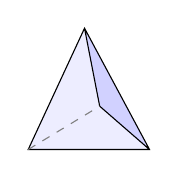
\begin{tikzpicture}[x=.55cm,y=.55cm]
 \fill[blue!7] (0,0)--(2.8,0)--(1.3,2.8)--cycle;
 \fill[blue!18] (2.8,0)--(1.65,1)--(1.3,2.8)--cycle;
 \draw (0,0)--(2.8,0)--(1.3,2.8)--cycle (2.8,0)--(1.65,1)--(1.3,2.8);
 \draw[dashed,gray] (0,0)--(1.65,1);
 \end{tikzpicture}}
\newcommand{\octa}{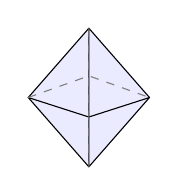
\begin{tikzpicture}[x=.55cm,y=.55cm]
 \fill[blue!8] (0,1.6)--(1.4,3.2)--(2.8,1.6)--(1.4,0)--cycle;
 \draw (0,1.6)--(1.4,3.2)--(2.8,1.6)--(1.4,0)--cycle (1.4,3.2)--(1.4,1.15)--(1.4,0) (0,1.6)--(1.4,1.15)--(2.8,1.6);
 \draw[dashed,gray] (1.4,3.2)--(1.4,2.1)--(1.4,0) (0,1.6)--(1.4,2.1)--(2.8,1.6);
 \end{tikzpicture}}
\newcommand{\prism}{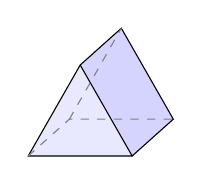
\begin{tikzpicture}[x=.55cm,y=.55cm]
 \fill[blue!9] (0,0)--(2.4,0)--(1.2,2.1)--cycle;
 \fill[blue!17] (2.4,0)--(3.35,.85)--(2.15,2.95)--(1.2,2.1)--cycle;
 \draw (0,0)--(2.4,0)--(1.2,2.1)--cycle (2.4,0)--(3.35,.85)--(2.15,2.95)--(1.2,2.1);
 \draw[dashed,gray] (0,0)--(.95,.85)--(3.35,.85) (.95,.85)--(2.15,2.95);
 \end{tikzpicture}}
\newcommand{\pyramid}{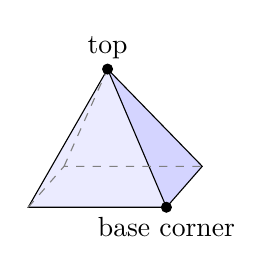
\begin{tikzpicture}[x=.65cm,y=.65cm]
 \fill[blue!8] (0,0)--(2.7,0)--(1.55,2.7)--cycle;
 \fill[blue!17] (2.7,0)--(3.4,.8)--(1.55,2.7)--cycle;
 \draw (0,0)--(2.7,0)--(3.4,.8)--(1.55,2.7)--cycle (2.7,0)--(1.55,2.7);
 \draw[dashed,gray] (0,0)--(.7,.8)--(3.4,.8) (.7,.8)--(1.55,2.7);
 \fill (1.55,2.7) circle (2pt);\node[above] at (1.55,2.7) {top};
 \fill (2.7,0) circle (2pt);\node[below] at (2.7,0) {base corner};
 \end{tikzpicture}}
\newcommand{\circleblank}[1]{\begin{tikzpicture}[x=1cm,y=1cm]
 \draw[gray!60] (0,0) circle (1.9);\fill (0,0) circle (1.4pt);\node[below] at (0,-2.05) {#1};\end{tikzpicture}}
\newcommand{\turnexample}{\begin{tikzpicture}[x=1cm,y=1cm,font=\small]
 \draw[fill=blue!10] (-.8,0)--(.1,0)--(-.35,.7794)--cycle;
 \draw[fill=blue!10] (.35,0)--(1.25,0)--(.8,.7794)--cycle;
 \fill (-.8,0) circle (1.4pt);\fill (.35,0) circle (1.4pt);
 \node at (.2,-.5) {two triangle corners};
 \draw[-{Latex}] (1.7,.3)--(2.3,.3);
 \begin{scope}[shift={(3.9,.3)}]
  \draw[gray!55] (0,0) circle (1.08);
  \draw[fill=blue!10] (0,0)--(1,0)--(.5,.866)--cycle;
  \fill (0,0) circle (1.4pt);\node at (0,-1.5) {one corner placed};
 \end{scope}
 \draw[-{Latex}] (5.3,.3)--(5.9,.3);
 \begin{scope}[shift={(7.5,.3)}]
  \draw[gray!55] (0,0) circle (1.08);
  \draw[fill=blue!10] (0,0)--(1,0)--(.5,.866)--cycle;
  \draw[fill=blue!10] (0,0)--(.5,.866)--(-.5,.866)--cycle;
  \draw[very thick,gray!65] (120:1.08) arc (120:360:1.08);
  \fill (0,0) circle (1.4pt);\node at (0,-1.5) {gap between free sides};
 \end{scope}
\end{tikzpicture}}

\begin{document}
<<body>>
\end{document}
